% Options for packages loaded elsewhere
% Options for packages loaded elsewhere
\PassOptionsToPackage{unicode}{hyperref}
\PassOptionsToPackage{hyphens}{url}
\PassOptionsToPackage{dvipsnames,svgnames,x11names}{xcolor}
%
\documentclass[
  english,
  11pt,
]{article}
\usepackage{xcolor}
\usepackage[margin=25mm]{geometry}
\usepackage{amsmath,amssymb}
\setcounter{secnumdepth}{-\maxdimen} % remove section numbering
\usepackage{iftex}
\ifPDFTeX
  \usepackage[T1]{fontenc}
  \usepackage[utf8]{inputenc}
  \usepackage{textcomp} % provide euro and other symbols
\else % if luatex or xetex
  \usepackage{unicode-math} % this also loads fontspec
  \defaultfontfeatures{Scale=MatchLowercase}
  \defaultfontfeatures[\rmfamily]{Ligatures=TeX,Scale=1}
\fi
\usepackage{lmodern}
\ifPDFTeX\else
  % xetex/luatex font selection
\fi
% Use upquote if available, for straight quotes in verbatim environments
\IfFileExists{upquote.sty}{\usepackage{upquote}}{}
\IfFileExists{microtype.sty}{% use microtype if available
  \usepackage[]{microtype}
  \UseMicrotypeSet[protrusion]{basicmath} % disable protrusion for tt fonts
}{}
\makeatletter
\@ifundefined{KOMAClassName}{% if non-KOMA class
  \IfFileExists{parskip.sty}{%
    \usepackage{parskip}
  }{% else
    \setlength{\parindent}{0pt}
    \setlength{\parskip}{6pt plus 2pt minus 1pt}}
}{% if KOMA class
  \KOMAoptions{parskip=half}}
\makeatother
% Make \paragraph and \subparagraph free-standing
\makeatletter
\ifx\paragraph\undefined\else
  \let\oldparagraph\paragraph
  \renewcommand{\paragraph}{
    \@ifstar
      \xxxParagraphStar
      \xxxParagraphNoStar
  }
  \newcommand{\xxxParagraphStar}[1]{\oldparagraph*{#1}\mbox{}}
  \newcommand{\xxxParagraphNoStar}[1]{\oldparagraph{#1}\mbox{}}
\fi
\ifx\subparagraph\undefined\else
  \let\oldsubparagraph\subparagraph
  \renewcommand{\subparagraph}{
    \@ifstar
      \xxxSubParagraphStar
      \xxxSubParagraphNoStar
  }
  \newcommand{\xxxSubParagraphStar}[1]{\oldsubparagraph*{#1}\mbox{}}
  \newcommand{\xxxSubParagraphNoStar}[1]{\oldsubparagraph{#1}\mbox{}}
\fi
\makeatother


\usepackage{longtable,booktabs,array}
\newcounter{none} % for unnumbered tables
\usepackage{calc} % for calculating minipage widths
% Correct order of tables after \paragraph or \subparagraph
\usepackage{etoolbox}
\makeatletter
\patchcmd\longtable{\par}{\if@noskipsec\mbox{}\fi\par}{}{}
\makeatother
% Allow footnotes in longtable head/foot
\IfFileExists{footnotehyper.sty}{\usepackage{footnotehyper}}{\usepackage{footnote}}
\makesavenoteenv{longtable}
\usepackage{graphicx}
\makeatletter
\newsavebox\pandoc@box
\newcommand*\pandocbounded[1]{% scales image to fit in text height/width
  \sbox\pandoc@box{#1}%
  \Gscale@div\@tempa{\textheight}{\dimexpr\ht\pandoc@box+\dp\pandoc@box\relax}%
  \Gscale@div\@tempb{\linewidth}{\wd\pandoc@box}%
  \ifdim\@tempb\p@<\@tempa\p@\let\@tempa\@tempb\fi% select the smaller of both
  \ifdim\@tempa\p@<\p@\scalebox{\@tempa}{\usebox\pandoc@box}%
  \else\usebox{\pandoc@box}%
  \fi%
}
% Set default figure placement to htbp
\def\fps@figure{htbp}
\makeatother



\ifLuaTeX
\usepackage[bidi=basic,shorthands=off]{babel}
\else
\usepackage[bidi=default,shorthands=off]{babel}
\fi
\ifLuaTeX
  \usepackage{selnolig} % disable illegal ligatures
\fi


\setlength{\emergencystretch}{3em} % prevent overfull lines

\providecommand{\tightlist}{%
  \setlength{\itemsep}{0pt}\setlength{\parskip}{0pt}}



 


\makeatletter
\@ifpackageloaded{caption}{}{\usepackage{caption}}
\AtBeginDocument{%
\ifdefined\contentsname
  \renewcommand*\contentsname{Table of contents}
\else
  \newcommand\contentsname{Table of contents}
\fi
\ifdefined\listfigurename
  \renewcommand*\listfigurename{List of Figures}
\else
  \newcommand\listfigurename{List of Figures}
\fi
\ifdefined\listtablename
  \renewcommand*\listtablename{List of Tables}
\else
  \newcommand\listtablename{List of Tables}
\fi
\ifdefined\figurename
  \renewcommand*\figurename{Figure}
\else
  \newcommand\figurename{Figure}
\fi
\ifdefined\tablename
  \renewcommand*\tablename{Table}
\else
  \newcommand\tablename{Table}
\fi
}
\@ifpackageloaded{float}{}{\usepackage{float}}
\floatstyle{ruled}
\@ifundefined{c@chapter}{\newfloat{codelisting}{h}{lop}}{\newfloat{codelisting}{h}{lop}[chapter]}
\floatname{codelisting}{Listing}
\newcommand*\listoflistings{\listof{codelisting}{List of Listings}}
\makeatother
\makeatletter
\makeatother
\makeatletter
\@ifpackageloaded{caption}{}{\usepackage{caption}}
\@ifpackageloaded{subcaption}{}{\usepackage{subcaption}}
\makeatother
\usepackage{bookmark}
\IfFileExists{xurl.sty}{\usepackage{xurl}}{} % add URL line breaks if available
\urlstyle{same}
% fallback for those not using the hyperref driver hyperxmp:
\makeatletter
\@ifundefined{xmpquote}{\newcommand{\xmpquote}[1]{#1}}{}
\makeatother
\hypersetup{
  pdftitle={How small does a collapsing vortex become?},
  pdflang={en},
  colorlinks=true,
  linkcolor={blue},
  filecolor={Maroon},
  citecolor={Blue},
  urlcolor={Blue},
  pdfcreator={LaTeX via pandoc}}


\title{How small does a collapsing vortex become?}
\usepackage{etoolbox}
\makeatletter
\providecommand{\subtitle}[1]{% add subtitle to \maketitle
  \apptocmd{\@title}{\par {\large #1 \par}}{}{}
}
\makeatother
\subtitle{Core size, extreme speeds, and the first limits of fluid
modelling}
\author{}
\date{2026-09-11}
\begin{document}
\maketitle


With an \textbf{illustrative} reference radius of 1 millimetre at a
characteristic speed of 1 metre per second, the inverse-law estimate
puts the core near \textbf{0.334 nanometres at one percent of the speed
of light}. That is comparable to the spacing between water molecules.
But familiar fluid approximations become questionable much earlier in
this example, while the core is still micrometres across in radius.

This article derives that estimate, explains its calibration, and asks
which physical assumptions should be checked first. It evaluates a
leading-order scaling model. It does not simulate a real collapsing
fluid or independently verify the proposed proof.

\subsection{A shrinking ruler and a growing
speed}\label{a-shrinking-ruler-and-a-growing-speed}

Imagine a family of curves on graph paper. At each step the horizontal
ruler gets smaller while the vertical ruler gets larger. The curves can
retain the same shape in their own units even though their physical
dimensions change enormously. Similarity variables make this idea
precise.

Write \(\tau>0\) for nondimensional time remaining. The paper's Section
2.1 gives characteristic scales

\[
r_c\asymp\tau^{1/2},\qquad
U\asymp\tau^{-(1/2+h)},\qquad 0<h<0.01.
\]

Here \(U\) is the dominant azimuthal or axial speed scale, rather than
the radial inflow speed or angular velocity. The symbol \(\asymp\) means
comparison up to fixed positive factors. The result concerns a
\textbf{forced incompressible} flow.
\href{https://cdn.openai.com/pdf/32d9f210-8b73-45e0-91bc-82a30aef8a9a/navier-stokes.pdf}{OpenAI,
Sections 1--2.1}

For a fixed profile and a consistently defined reference stage, model
the normalized scales as

\[
\frac{r_c}{r_0}=\left(\frac{\tau}{\tau_0}\right)^{1/2},
\qquad
\frac{U}{U_0}=\left(\frac{\tau}{\tau_0}\right)^{-(1/2+h)}.
\]

Solving the second relation for time and substituting into the first
gives

\[
\boxed{\frac{r_c}{r_0}=\left(\frac{U}{U_0}\right)^{-\alpha}},
\qquad \alpha=\frac{1}{1+2h}.
\]

These equalities define our power-law surrogate; they do not turn the
paper's comparison estimates into exact numerical profiles. At a fixed
nonzero similarity location, profile factors can cancel in a normalized
leading-field ratio. They must still be determined to attach physical
units.

The inverse formula is useful too:

\[
U(\ell)=U_0\left(\frac{r_0}{\ell}\right)^{1+2h}.
\]

This gives a \textbf{formal} speed at which the surrogate's radius
equals a selected length \(\ell\). A comparison with a radius should not
silently be described as a comparison with a diameter; the latter is
\(2r_c\).

\begin{figure}

\centering{

\pandocbounded{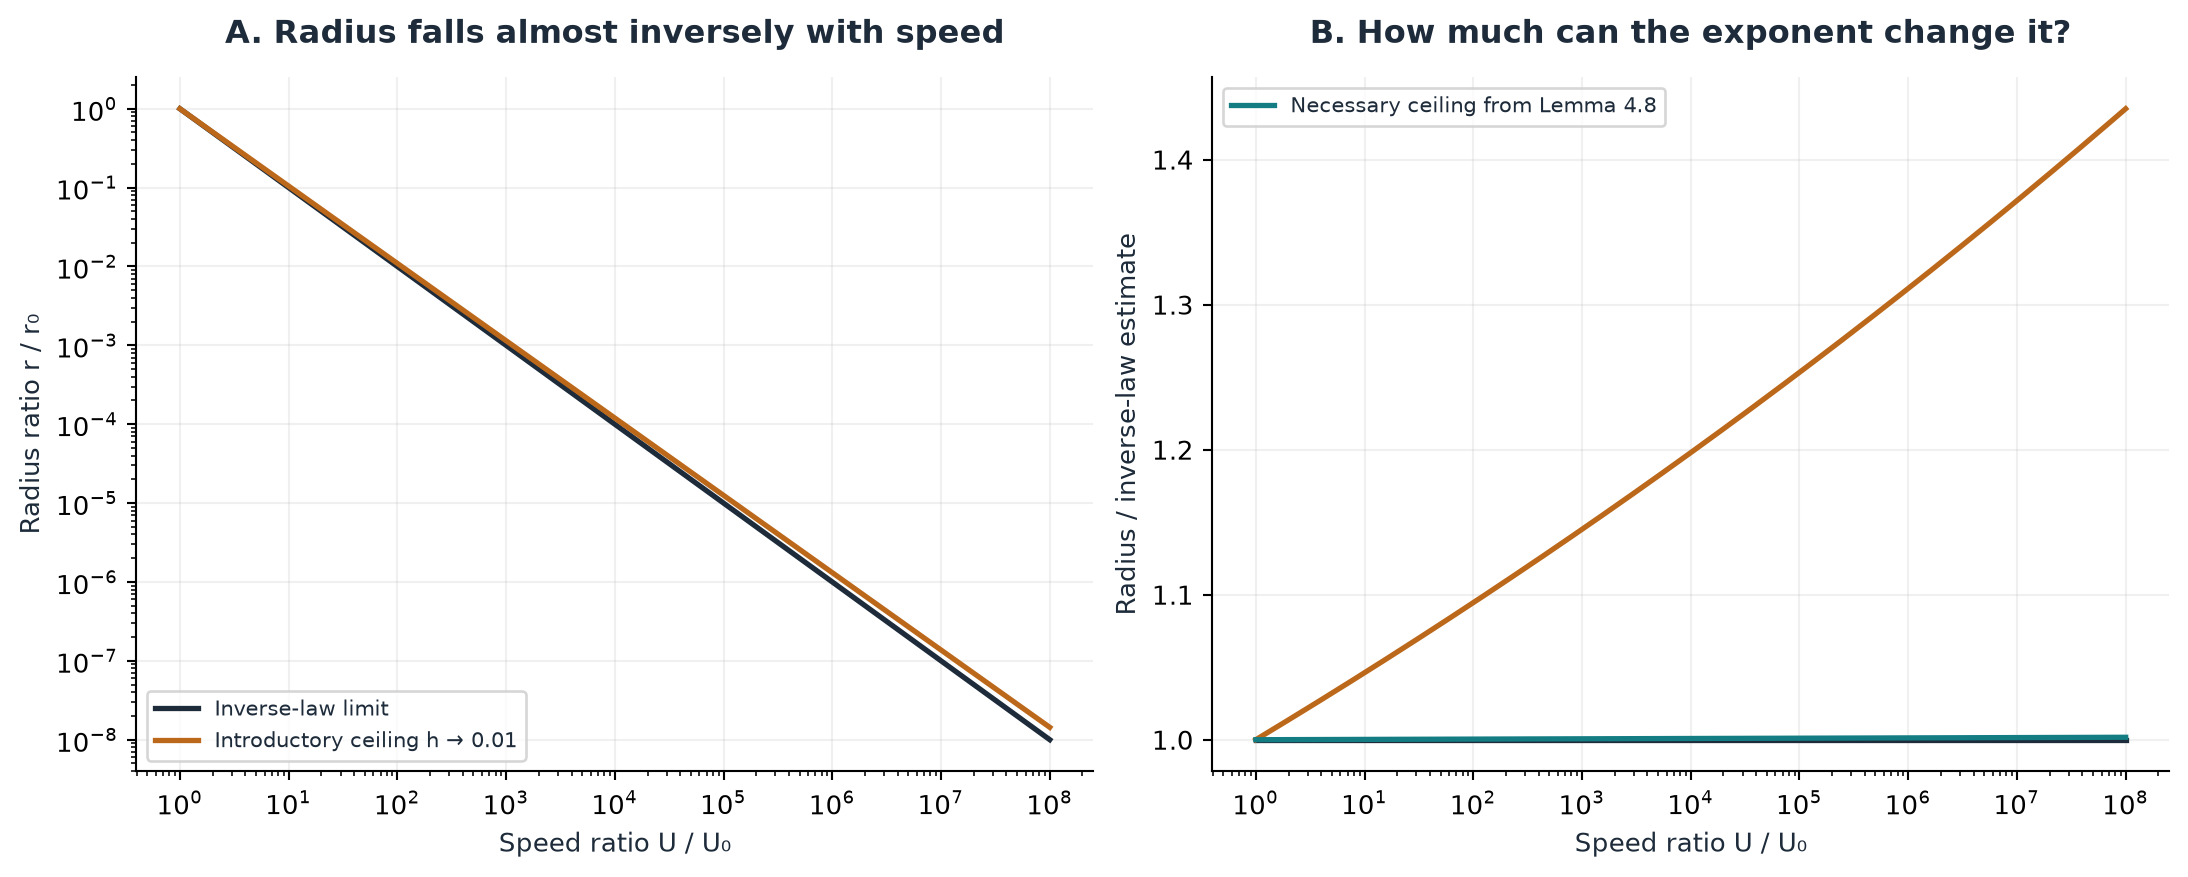
\includegraphics[keepaspectratio,alt={Two plots show radius falling almost inversely with speed and the much smaller exponent effect implied by the detailed parameter hierarchy.}]{figures/01_dimensionless_scaling.png}}

}

\caption{\label{fig-scaling}The normalized power law and its departure
from an inverse law. The orange curve uses the introductory limiting
ceiling; it is not an admissible profile choice.}

\end{figure}%

\subsection{Why use the inverse-law
limit?}\label{why-use-the-inverse-law-limit}

The parameter \(h\) is chosen with other construction parameters, not
freely fitted. Lemma 4.8, page 35, requires \(h<e^{-T_d}\) with
\(T_d=e^{M_d}+10\). Since \(e^{M_d}>0\), a necessary ceiling is
\(h<e^{-10}\). Other requirements can make it smaller still.

We therefore use \textbf{\(h\to0^+\)}, or \(r_c\approx r_0U_0/U\), for
the headline calculation. The endpoint \(h=0\) is a limiting proxy, not
a theorem instance. With the reference pair below, the necessary ceiling
changes the radius at \(0.01c\) by less than \textbf{0.135 percent},
holding the anchor fixed. This is an exponent-only bound, not an
uncertainty bound on the actual flow. The wider \(0<h<0.01\) sweep is
retained solely to illustrate sensitivity.

\subsection{Putting metres on the
axes}\label{putting-metres-on-the-axes}

Choose \(r_0=10^{-3}\,\mathrm m\) and \(U_0=1\,\mathrm{m\,s^{-1}}\) at a
stage with nonzero velocity. The initially resting state cannot supply
that anchor.

To restore units consistently, let

\[
x=L_*\hat x,\quad t=t_*\hat t,\quad
u=\frac{L_*}{t_*}\hat u,\quad
\hat\nu=\nu\frac{t_*}{L_*^2}.
\]

For a construction with \(\hat\nu=1\), the unit scales obey
\(t_*=L_*^2/\nu\). Consequently, a physical reference pair must satisfy

\[
\frac{r_0U_0}{\nu}=\hat r_0\hat U_0.
\]

We have \textbf{not} determined the right-hand side from a complete
profile. Our millimetre/metre-per-second pair is an illustrative
calibration, not a demonstrated realization in air or water. There is
also no calibrated time-to-collapse in seconds.

{\def\LTcaptype{none} % do not increment counter
\begin{longtable}[]{@{}lll@{}}
\toprule\noalign{}
Speed marker & Speed (m/s) & Core radius, inverse-law limit \\
\midrule\noalign{}
\endhead
\bottomrule\noalign{}
\endlastfoot
Air Ma=0.3 screen & 103.5 & 9.66 µm \\
Air Ma=1 & 345 & 2.9 µm \\
Air Ma=5 marker & 1725 & 580 nm \\
Water Ma=0.3 screen & 449 & 2.23 µm \\
Water Ma=1 marker & 1497 & 668 nm \\
1 km/s & 1000 & 1 µm \\
0.01c (formal) & 2.998e+06 & 334 pm \\
0.1c (formal) & 2.998e+07 & 33.4 pm \\
\end{longtable}
}

The sonic markers use the reference sound speeds below. The high-speed
entries extrapolate far beyond those reference states' applicability. In
particular, the calculation predicts neither stable water at these
speeds nor an experimentally attainable route to them.

\begin{figure}

\centering{

\pandocbounded{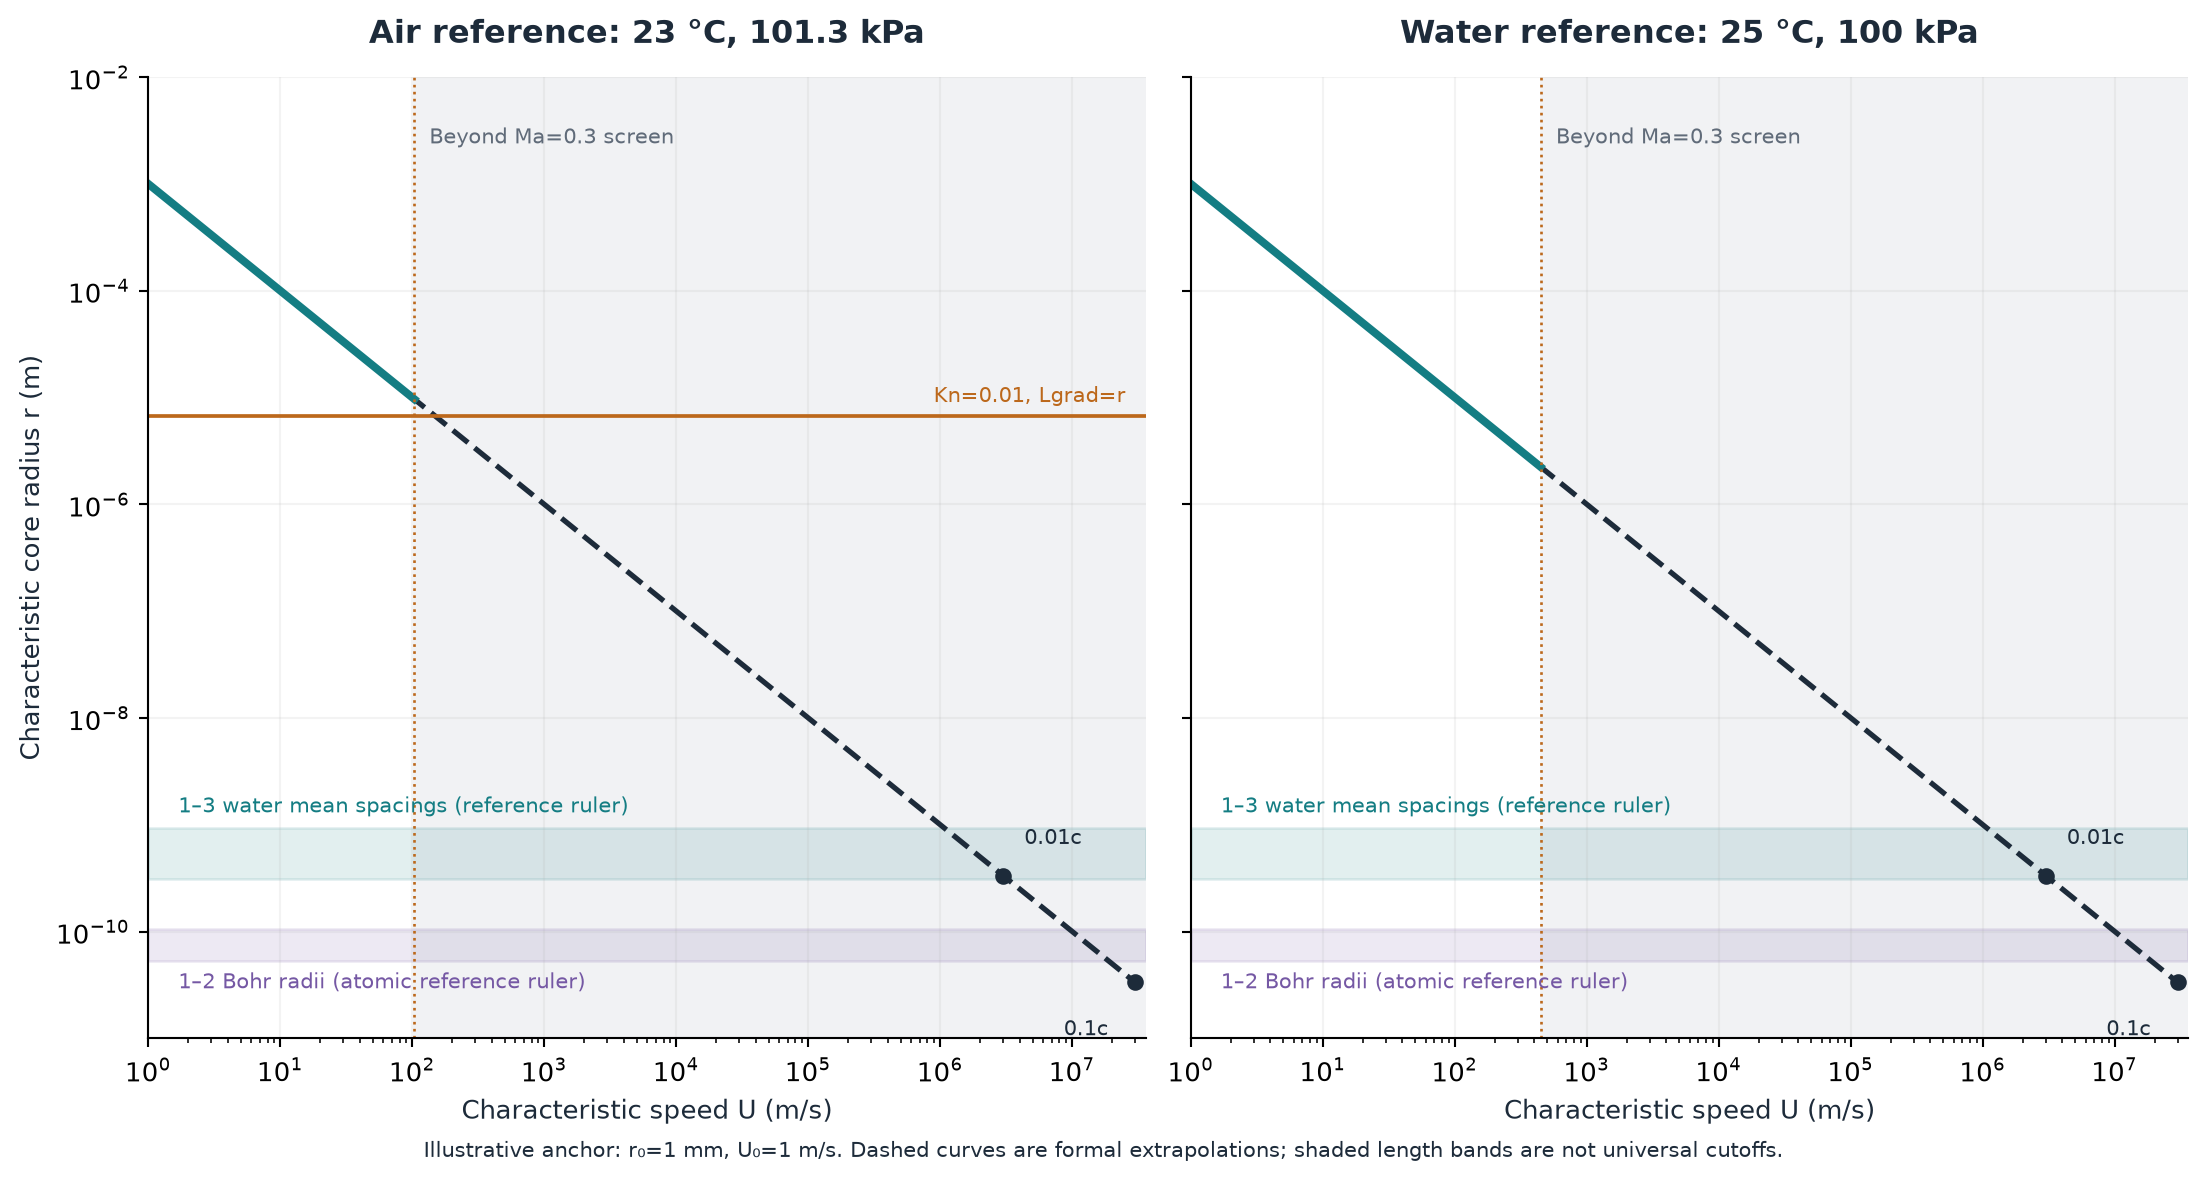
\includegraphics[keepaspectratio,alt={Radius-versus-speed plots show micrometre-scale Mach screens, an air Knudsen screen, molecular-spacing rulers, and atomic reference rulers. Extreme-speed points lie on formal extrapolations.}]{figures/02_core_size_and_physical_scales.png}}

}

\caption{\label{fig-physical}The same illustrative scaling compared with
air and water reference properties. Grey regions are beyond a Mach
screening marker; teal segments only precede the displayed screens and
do not certify physical validity.}

\end{figure}%

\subsection{Which assumption needs attention
first?}\label{which-assumption-needs-attention-first}

\textbf{Compressibility.} Define \(Ma=U/c_s\), with a characteristic
speed relative to the vortex's bulk motion. A low-Mach screen near
\(0.3\) is a useful engineering convention, not a universal transition.
For our air reference it is reached near 103 m/s, at a radius near 9.66
micrometres. The same marker for water occurs near 2.23 micrometres.
Cavitation, heating, or other state changes could matter sooner; they
are not evaluated here.
\href{https://ntrs.nasa.gov/api/citations/19960045736/downloads/19960045736.pdf}{Low-Mach
modelling discussion}

\textbf{Gas continuum modelling.} A relevant diagnostic is
\(Kn=\lambda/L_{\rm grad}\). The NIST air reference gives
\(\lambda=67.3\) nm at 296.15 K and 101.3 kPa, using that study's
mean-free-path convention. We assume \(L_{\rm grad}=\beta r_c\), with
\(\beta=1\) as a proxy. A \(Kn=0.01\) screen then corresponds to
\(r_c=6.73\) micrometres and a formal speed near 149 m/s. Thus Mach
screening comes first \textbf{among these two screens under these
assumptions}. Taking \(\beta=0.1\) reverses their order.
\href{https://nvlpubs.nist.gov/nistpubs/jres/110/1/j110-1kim.pdf}{NIST,
Equation 11 and Table 3},
\href{https://ntrs.nasa.gov/api/citations/20000004526/downloads/20000004526.pdf}{NASA
discussion of Knudsen screening}

\textbf{Liquids and atomic scales.} For water, estimate the molecular
number density as \(n=\rho N_A/M\) and the mean spacing as
\(d=n^{-1/3}\). This gives 0.311 nm. It is a cubic mean-spacing
estimate, not a molecular diameter. The atomic ruler is the Bohr radius,
approximately 0.0529 nm, not the radius of every atom. A local flow
description needs an averaging length containing many molecules while
remaining small relative to its variation scale. Once those requirements
cannot be met, resolving this smooth local vortex as a classical
continuum loses its physical basis.
\href{https://iapws.org/technical-guidance/release/LiquidWater.download}{IAPWS
Table 8}, \href{https://webbook.nist.gov/cgi/cbook.cgi?Name=water}{NIST
water molar mass},
\href{https://physics.nist.gov/cuu/Constants/Table/allascii.txt}{CODATA
constants}

{\def\LTcaptype{none} % do not increment counter
\begin{longtable}[]{@{}lll@{}}
\toprule\noalign{}
Length used as radius & Length & Formal speed (m/s) \\
\midrule\noalign{}
\endhead
\bottomrule\noalign{}
\endlastfoot
Air Kn=0.01 radius proxy & 6.73 µm & 149 \\
Air mean free path & 67.3 nm & 1.49e+04 \\
Air mean spacing & 3.43 nm & 2.92e+05 \\
10 water mean spacings & 3.11 nm & 3.22e+05 \\
3 water mean spacings & 932 pm & 1.07e+06 \\
1 water mean spacing & 311 pm & 3.22e+06 \\
1 Bohr radius & 52.9 pm & 1.89e+07 \\
\end{longtable}
}

There is no single universal molecular cutoff. Some averaged transport
predictions agree with molecular simulations even at extremely small
confinement; that does not establish the validity of every local
velocity or stress field.
\href{https://arxiv.org/abs/1501.01476}{Gravelle and colleagues}

\subsection{What controls the
uncertainty?}\label{what-controls-the-uncertainty}

At fixed speed, the surrogate has logarithmic sensitivities

\[
\frac{\partial\log r_c}{\partial\log r_0}=1,\qquad
\frac{\partial\log r_c}{\partial\log U_0}=\alpha.
\]

A factor of ten in either reference scale changes the inferred radius by
approximately a factor of ten. Uncertainty in the radius normalization
is mathematically indistinguishable from uncertainty in \(r_0\) here; it
should not be counted again as an independent error bar.

\begin{figure}

\centering{

\pandocbounded{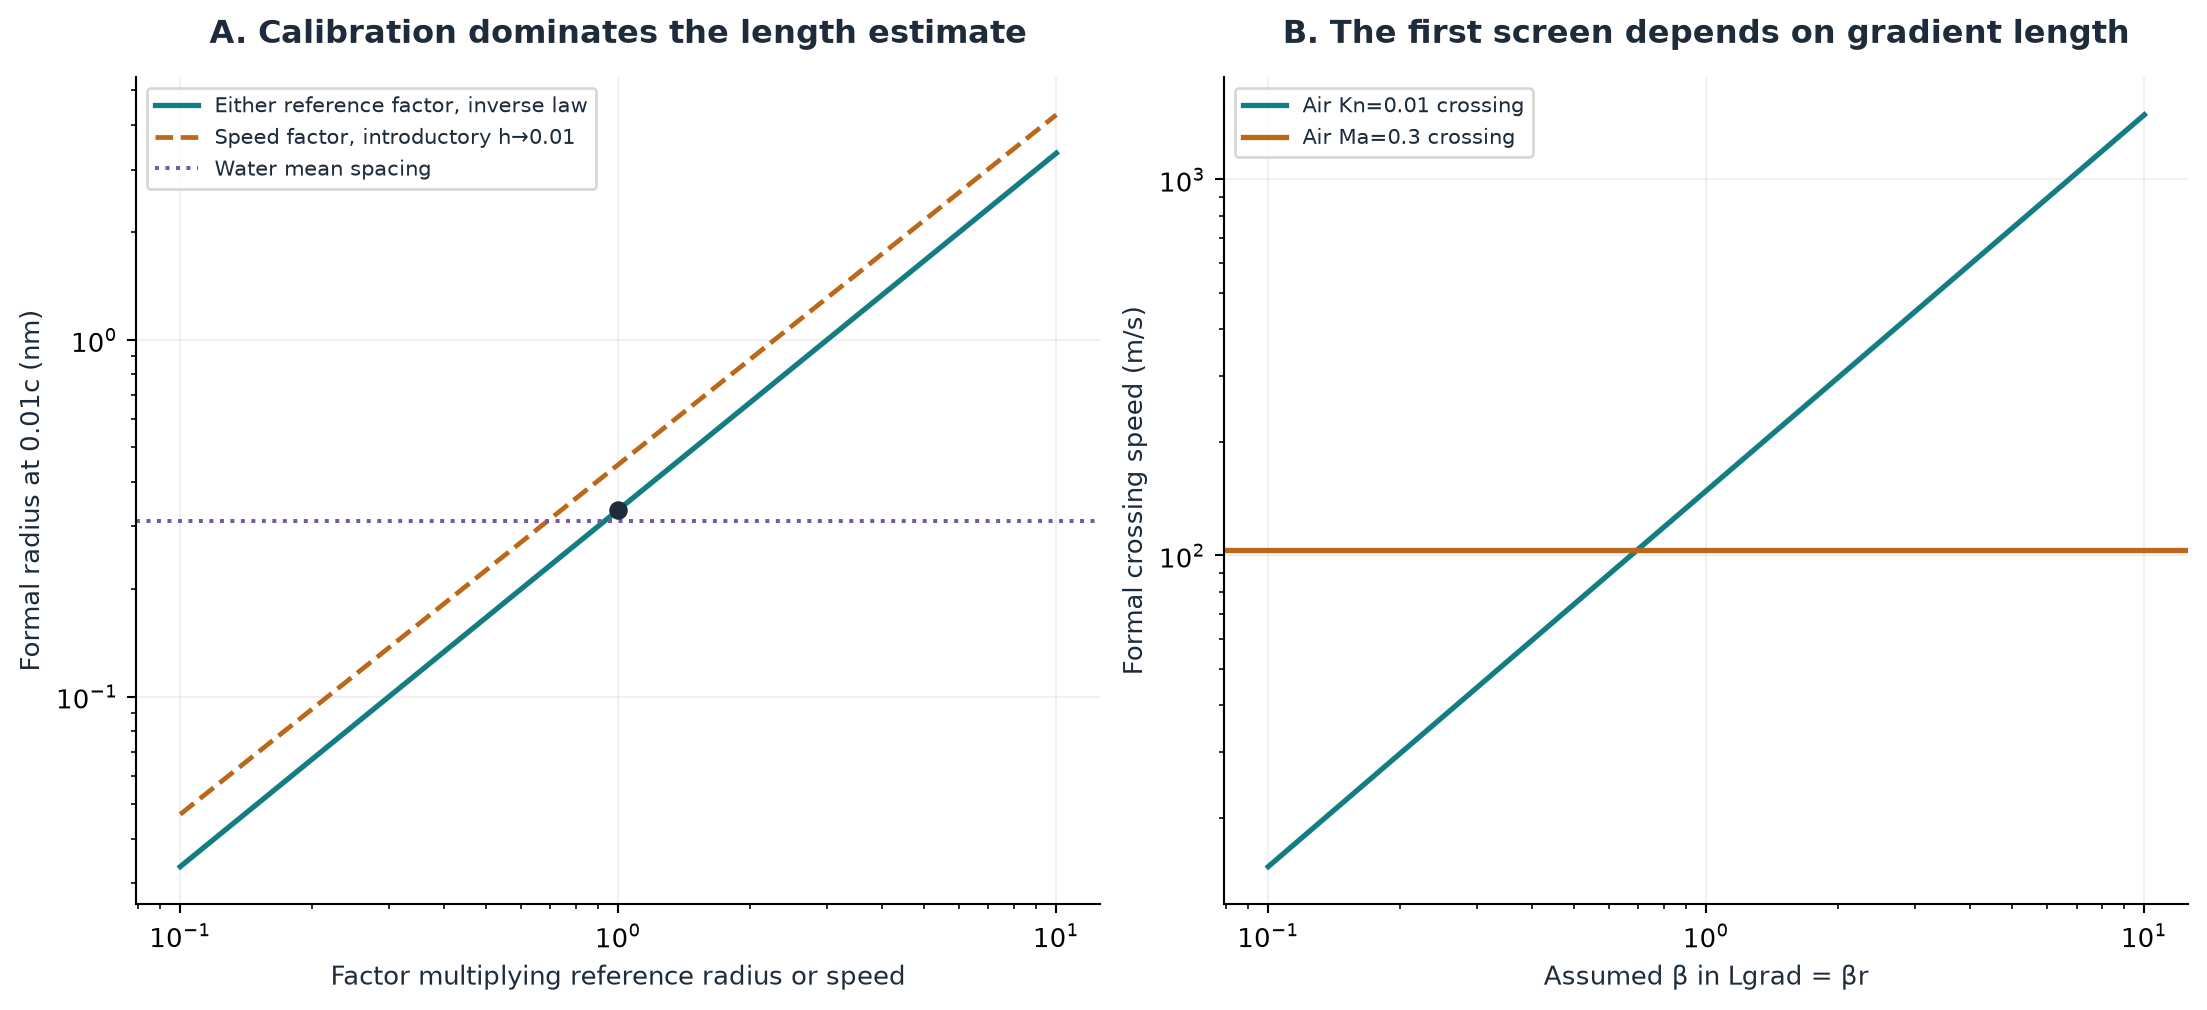
\includegraphics[keepaspectratio,alt={Changing the reference calibration moves the molecular-scale prediction substantially. A second panel shows the Knudsen crossing moving across the fixed Mach crossing as the gradient-length proxy changes.}]{figures/03_calibration_and_gradient_sensitivity.png}}

}

\caption{\label{fig-sensitivity}Reference-scale sensitivity at 0.01c,
and the competing air screens as the assumed gradient length changes.
The orange exponent example is illustrative and violates the detailed
necessary ceiling.}

\end{figure}%

The property values are frozen reference markers, not a thermodynamic
evolution:

{\def\LTcaptype{none} % do not increment counter
\begin{longtable}[]{@{}lll@{}}
\toprule\noalign{}
Reference property & Air & Liquid water \\
\midrule\noalign{}
\endhead
\bottomrule\noalign{}
\endlastfoot
Temperature / pressure & 296.15 K / 101.3 kPa & 298.15 K / 100 kPa \\
Density (kg/m³) & 1.192 (ideal gas) & 997.047 \\
Sound speed (m/s) & 345 (ideal gas) & 1496.7 \\
Kinematic viscosity (m²/s) & 1.538e-05 & 8.926e-07 \\
Mean spacing n\^{}(-1/3) & 3.43 nm & 311 pm \\
Mean free path & 67.3 nm & Not assigned a dilute-gas value \\
\end{longtable}
}

The air density and sound speed use the ideal-gas estimates
\(\rho=p/(RT)\) and \(c_s=\sqrt{\gamma RT}\) with rounded assumptions
\(R=287.05\) J/(kg K) and \(\gamma=1.4\). Viscosities and the water
sound speed come from the listed reference tables.
\href{https://www.grc.nasa.gov/www/k-12/BGP/snddrv.html}{Ideal-gas
sound-speed derivation}

\subsection{What this calculation
establishes}\label{what-this-calculation-establishes}

The algebra explains the nearly inverse radius-speed relation, and the
explicit calibration shows how an extreme-speed extrapolation reaches
molecular scales. In the example, the displayed Mach and gas continuum
screens intervene at much larger radii.

The remaining physical questions include the actual gradient field,
pressure and temperature evolution, liquid relaxation times, and the
correction pulses' potentially shorter spatial and temporal scales. A
collision-time proxy for air can be estimated from \(\lambda/\bar v\),
but it does not supply the uncomputed strain field. No CFD grid is used,
and no conclusion about full-proof validity or dynamical stability
follows from these calculations.

The \href{source-notes.md}{source and calibration notes} document the
definitions and unresolved quantities. The
\href{../../code/d1_core_size/study.ipynb}{executed notebook},
\href{../../code/d1_core_size/parameters.json}{parameter file}, and
\href{../../code/d1_core_size/data/}{CSV data} support reproduction. The
next article will explain how a growing velocity can coexist with
bounded energy.




\end{document}
